\newcounter{english}
\documentclass{article}

% packages
\usepackage{amsmath, amsthm, thmtools, amsfonts, amssymb, luacode, catchfile, tikzducks, hyperref, ifthen}
\ifcsname c@kobocompile\endcsname
	\usepackage[a5paper, total={1072pt, 1448pt}, margin=10pt, includeheadfoot]{geometry} % set page margins
\else
	\usepackage[a4paper, margin=50pt, includeheadfoot]{geometry}
\fi
\usepackage[shortlabels]{enumitem}
\usepackage[skip=3pt, indent=0pt]{parskip}

% language
\usepackage[bidi=basic, layout=tabular, provide=*]{babel}
\ifcsname c@english\endcsname
	\babelprovide[main, import]{english}
\else
	\babelprovide[main, import]{hebrew}
	\babelprovide{rl}
\fi
%\babelfont{rm}{Libertinus Serif}
\babelfont{rm}[Renderer=Harfbuzz]{Libertinus Serif}
\babelfont{sf}{Libertinus Sans}
\babelfont{tt}{Libertinus Mono}

% style
\AddToHook{cmd/section/before}{\clearpage}	% Add line break before section
\linespread{1.3}
\setcounter{secnumdepth}{0}		% Remove default number tags from sections, this won't do well with theorems
\AtBeginDocument{\setlength{\belowdisplayskip}{3pt}}
\AtBeginDocument{\setlength{\abovedisplayskip}{3pt}}
\graphicspath{ {../images/} }

% operators
\DeclareMathOperator\cis{cis}
\DeclareMathOperator\Sp{Sp}
\DeclareMathOperator\tr{tr}
\DeclareMathOperator\im{Im}
\DeclareMathOperator\re{Re}
\DeclareMathOperator\diag{diag}
\DeclareMathOperator*\lowlim{\underline{lim}}
\DeclareMathOperator*\uplim{\overline{lim}}
\DeclareMathOperator\rng{rng}
\DeclareMathOperator\Sym{Sym}
\DeclareMathOperator\Arg{Arg}
\DeclareMathOperator\Log{Log}
\DeclareMathOperator\dom{dom}
\DeclareMathOperator\supp{Supp}
\DeclareMathOperator\var{Var}
\DeclareMathOperator\cov{Cov}

% commands
%\renewcommand\qedsymbol{\textbf{מש''ל}}
%\renewcommand\qedsymbol{\fbox{\emoji{lizard}}}
\newcommand{\Aa}[0]{\mathcal{A}}
\newcommand{\Bb}[0]{\mathcal{B}}
\newcommand{\CC}[0]{\mathbb{C}}
\newcommand{\Cc}[0]{\mathcal{C}}
\newcommand{\EE}[0]{\mathbb{E}}
\newcommand{\FF}[0]{\mathbb{F}}
\newcommand{\Ff}[0]{\mathcal{F}}
\newcommand{\Ii}[0]{\mathcal{I}}
\newcommand{\Gg}[0]{\mathcal{G}}
\newcommand{\Ll}[0]{\mathcal{L}}
\newcommand{\Mm}[0]{\mathcal{M}}
\newcommand{\NN}[0]{\mathbb{N}}
\newcommand{\Nn}[0]{\mathcal{N}}
\newcommand{\PP}[0]{\mathbb{P}}
\newcommand{\Pp}[0]{\mathcal{P}}
\newcommand{\QQ}[0]{\mathbb{Q}}
\newcommand{\RR}[0]{\mathbb{R}}
\newcommand{\Rr}[0]{\mathcal{R}}
\newcommand{\Ss}[0]{\mathcal{S}}
\newcommand{\TT}[0]{\mathbb{T}}
\newcommand{\Uu}[0]{\mathcal{U}}
\newcommand{\Vv}[0]{\mathcal{V}}
\newcommand{\Ww}[0]{\mathcal{W}}
\newcommand{\ZZ}[0]{\mathbb{Z}}
\newcommand{\acts}[0]{\circlearrowright}
\newcommand{\explain}[2] {
	\begin{flalign*}
		 && \text{#2} && \text{#1}
	\end{flalign*}
}
\newcommand{\maketitleprint}[0]{ \begin{center}
	%\begin{tikzpicture}[scale=3]
	%	\duck[graduate=gray!20!black, tassel=red!70!black]
	%\end{tikzpicture}	
	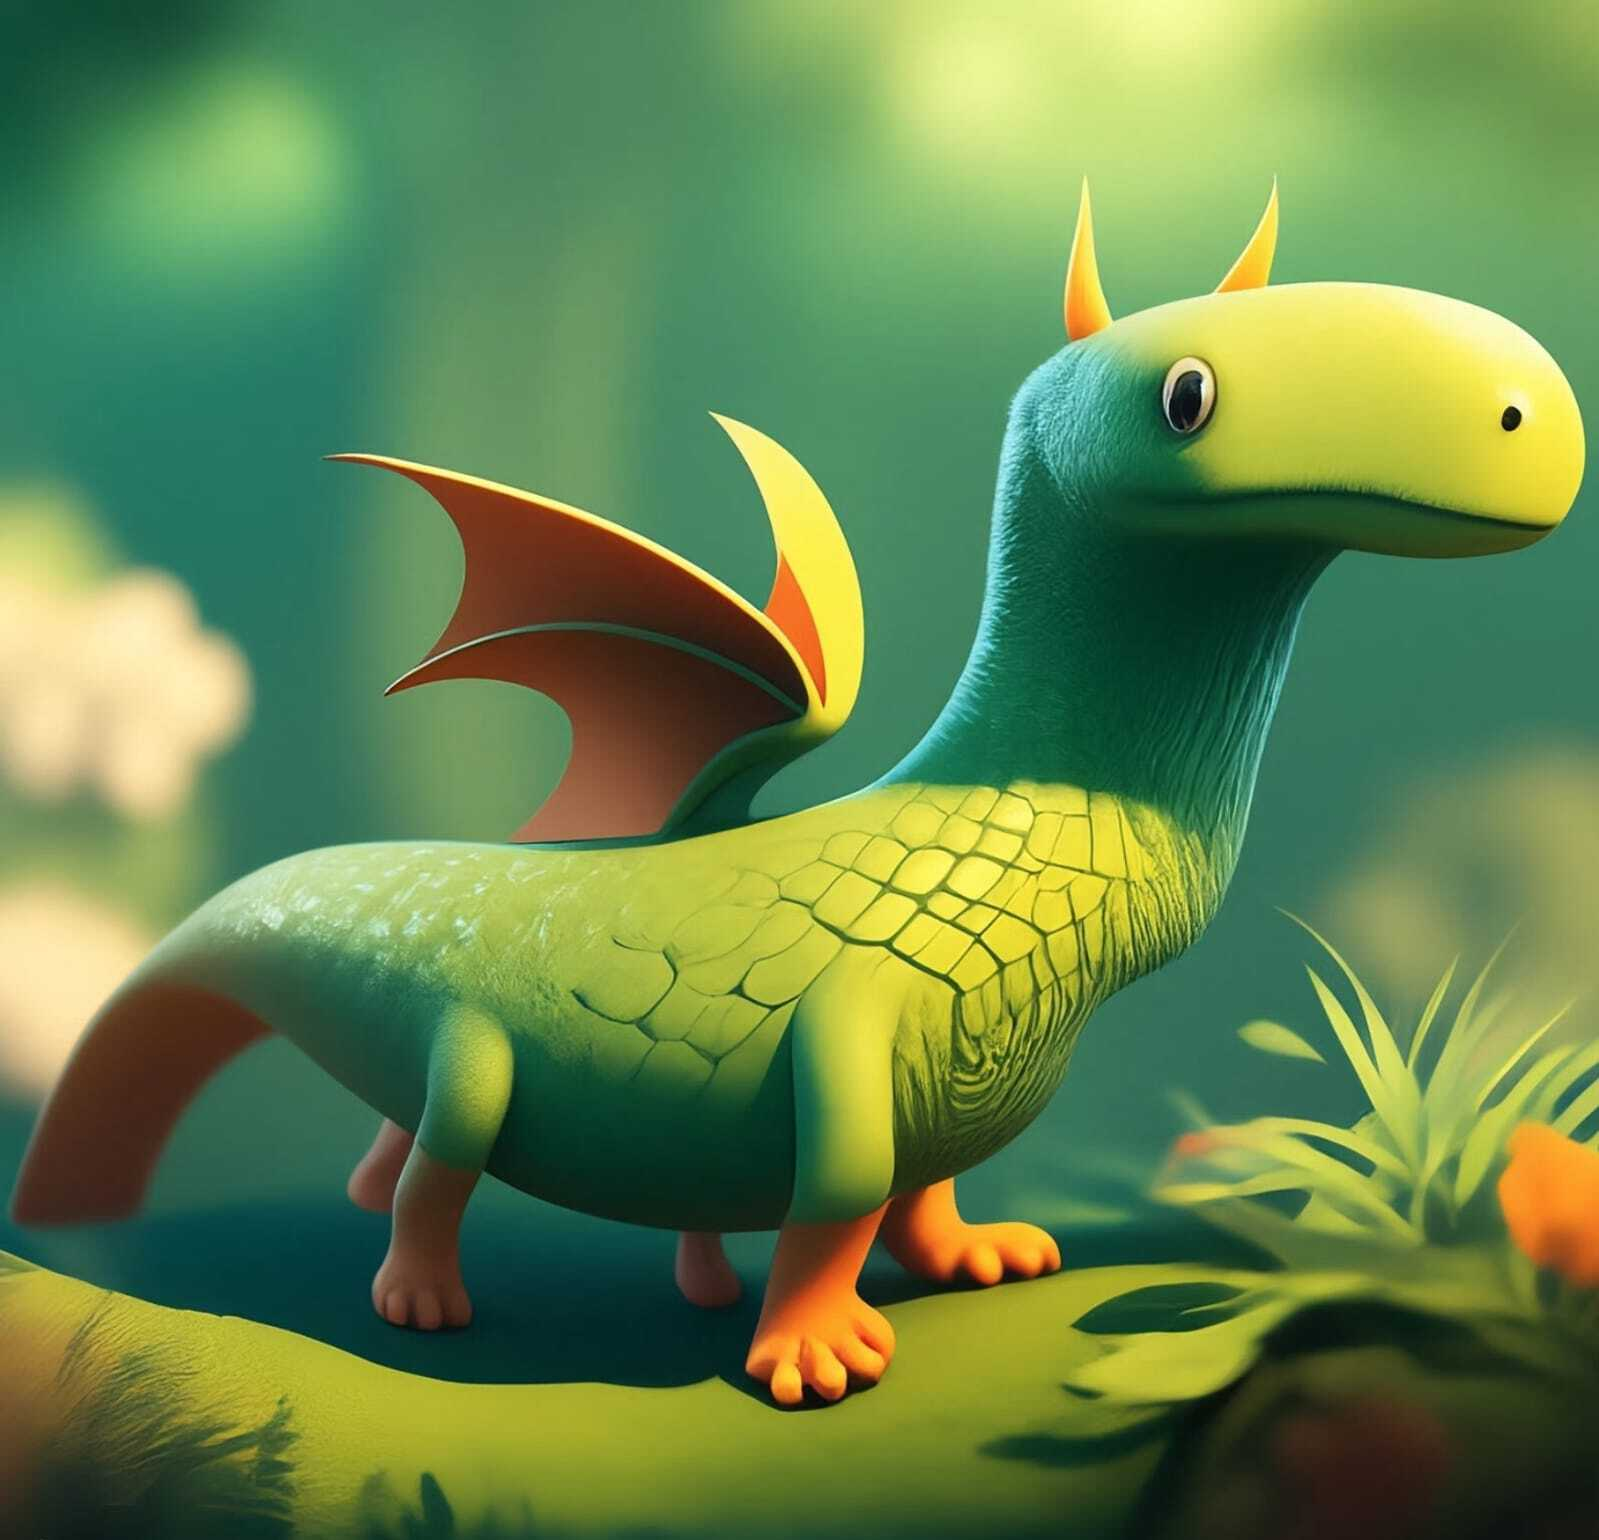
\includegraphics[width=6cm]{cover}
\end{center}
}

% theorem commands
\newtheoremstyle{c_remark}
	{}	% Space above
	{}	% Space below
	{}% Body font
	{}	% Indent amount
	{\bfseries}	% Theorem head font
	{}	% Punctuation after theorem head
	{.5em}	% Space after theorem head
	{\thmname{#1}\thmnumber{ #2}\thmnote{ \normalfont{\text{(#3)}}}}	% head content
\newtheoremstyle{c_definition}
	{3pt}	% Space above
	{3pt}	% Space below
	{}% Body font
	{}	% Indent amount
	{\bfseries}	% Theorem head font
	{}	% Punctuation after theorem head
	{.5em}	% Space after theorem head
	{\thmname{#1}\thmnumber{ #2}\thmnote{ \normalfont{\text{(#3)}}}}	% head content
\newtheoremstyle{c_plain}
	{3pt}	% Space above
	{3pt}	% Space below
	{\itshape}% Body font
	{}	% Indent amount
	{\bfseries}	% Theorem head font
	{}	% Punctuation after theorem head
	{.5em}	% Space after theorem head
	{\thmname{#1}\thmnumber{ #2}\thmnote{ \text{(#3)}}}	% head content

\ifcsname c@english\endcsname
	\theoremstyle{plain}
	\newtheorem{theorem}{Theorem}[section]
	\newtheorem{lemma}[theorem]{Lemma}
	\newtheorem{proposition}[theorem]{Proposition}
	\newtheorem*{proposition*}{Proposition}
	%\newtheorem{corollary}[theorem]{אין חלופה עברית}

	\theoremstyle{definition}
	\newtheorem{definition}[theorem]{Definition}
	\newtheorem*{definition*}{Definition}
	\newtheorem{example}{Example}[section]
	\newtheorem{exercise}{Exercise}[section]

	\theoremstyle{remark}
	\newtheorem*{remark}{Remark}
	\newtheorem*{solution}{Solution}
	\newtheorem{conclusion}[theorem]{Conclusion}
	\newtheorem{notation}[theorem]{Notation}
\else
	\theoremstyle{c_plain}
	\newtheorem{theorem}{משפט}[section]
	\newtheorem{lemma}[theorem]{למה}
	\newtheorem{proposition}[theorem]{טענה}
	\newtheorem*{proposition*}{טענה}
	%\newtheorem{corollary}[theorem]{אין חלופה עברית}

	\theoremstyle{c_definition}
	\newtheorem{definition}[theorem]{הגדרה}
	\newtheorem*{definition*}{הגדרה}
	\newtheorem{example}{דוגמה}[section]
	\newtheorem{exercise}{תרגיל}[section]

	\theoremstyle{c_remark}
	\newtheorem*{remark}{הערה}
	\newtheorem*{solution}{פתרון}
	\newtheorem{conclusion}[theorem]{מסקנה}
	\newtheorem{notation}[theorem]{סימון}
\fi

% Questions related commands
\newcounter{question}
\setcounter{question}{1}
\newcounter{sub_question}
\setcounter{sub_question}{1}

\ifcsname c@english\endcsname
	\newcommand{\question}[1][0]{
		\ifthenelse{#1 = 0}{}{\setcounter{question}{#1}}
		\section{Question \arabic{question}}
		\addtocounter{question}{1}
		\setcounter{sub_question}{1}
	}

	\newcommand{\subquestion}[1][0]{
		\ifthenelse{#1 = 0}{}{\setcounter{sub_question}{#1}}
		\subsection{Part \alph{sub_question}}
		\addtocounter{sub_question}{1}
	}
\else
	\newcommand{\question}[1][0]{
		\ifthenelse{#1 = 0}{}{\setcounter{question}{#1}}
		\section{שאלה \arabic{question}}
		\addtocounter{question}{1}
		\setcounter{sub_question}{1}
	}

	\newcommand{\subquestion}[1][0]{
		\ifthenelse{#1 = 0}{}{\setcounter{sub_question}{#1}}
		\subsection{סעיף \localecounter{letters.gershayim}{sub_question}}
		\addtocounter{sub_question}{1}
	}
\fi

% import lua and start of document
\directlua{common = require ('../common')}

\GetEnv{AUTHOR}

% headers
\author{\AUTHOR}
\date\today

\title{Solution to Exercise 0 --- Model Theory (1), 80616}

\begin{document}
\maketitle
\maketitleprint[yellow]

\question{}
Let $L = \{ P \}$ a language where $P$ is unary relation.
Define,
\[
	\varphi_n
	= \exists x_0 \ldots \exists x_n \left( \bigwedge_{i \le n} P(x_i) \land \bigwedge_{i < j \le n} x_i \ne x_j \right),
	\quad
	\psi_n
	= \exists x_0 \ldots \exists x_n \left( \bigwedge_{i \le n} \lnot P(x_i) \land \bigwedge_{i < j \le n} x_i \ne x_j \right)
\]
and let $T = \{ \varphi_n, \psi_n \mid n < \omega \}$. \\
We will show that $\cl_{\vdash} T$ is $\omega$-categoric.
\begin{proof}
	Let us define the model $\Mm \models T$ such that $M = 2 \times \NN$ and $\langle 0, n \rangle \in P^\Mm$ for $n < \omega$, as well $\langle 0, n \rangle \notin P^\Mm$.
	It is clear that for any $n$, we can choose $\langle \langle 0, i \rangle \mid i < n \rangle$ as witnesses for $\varphi_n$, and similarly choose $\langle 1, i \rangle$ for $\psi_n$. \\
	Let $\Nn \models T$ be some countable model, we will show that $\Nn \cong \Mm$.
	For $n = 0$, $\Nn \models \varphi_n \implies \Nn \models \exists x\ P(x)$, and let $f(0, 0) = x$, and in similar manner $f(1, 0) = y$ for the witness of $\psi_0 = \exists \lnot P(x)$.
	We use this as a basis for recursive definition of a function $f : M \to N$, it will be required to show in induction over $n$ that we can choose explicitly $x_i$ in $\varphi_n$ for $i < n$. \\
	Let us assume the induction and recursion step, meaning that $f \restriction 2 \times n$ is defined.
	$\Nn \models \varphi_{n + 1}$, meaning that there are at lest $n + 1$ elements of $\Nn$ such that they are in $P^\Nn$,
	by the pigeonhole principle there is at least one element $a \in N$ such that $f(0, k) \ne a$ for $k < n + 1$, then we can define $f(0, n + 1) = a$.
	This conclude our step, hence there is such function $f$, and by our construction it also holds that $f$ is embedding of $\Mm$ into $\Nn$, but 

	This is all irrelevant, I can just use the set definition of $\Nn$.
\end{proof}

\question{}
Let $L = \{ c_n \mid n < \omega \}$ be language consists of constant symbols.
Let us define the theory $T = \{ c_i \ne c_j \mid i < j < \omega \}$. \\
We will show that there are countably many non-isomorphic countable models of $T$, and that $T$ is complete.
\begin{proof}
	Let us define the model $\Mm_n$ such that $M = \omega$ and,
	\[
		c_i^\Mm = i + n
	\]
	for any $i < j < \omega$,
	\[
		c_i^\Mm
		= i + n
		\ne j + n
		= c_j^\Mm
	\]
	therefore $\Mm_n \models T$.
	$\Mm_n \models k \ne c_i$ for all $i < \omega$, in particular $\Mm_n \models \exists x\ x \ne c_i$.
	It is implied that also,
	\[
		\Mm_n
		\models \exists x_0 \ldots \exists x_{k - 1} \left( \bigwedge_{i < j < k} x_i \ne x_j \land x_i \ne c_l \right)
		= \varphi_l^k
	\]
	for all $l < \omega$.
	Finally, $\Mm_n \not\models \varphi_l^k$ for any $k > n$, we deduce that $\Mm_n \not\cong \Mm_m$ for any $n \ne m$.

	We move to show that $T$ is complete.
	Let us assume toward a contradiction that $\varphi$ is a sentence such that $\varphi \notin T$ and $T \cup \{ \varphi \}$ is consistent.
	By construction of Henkin models we can deduce that $\Mm_0 \models \varphi$, but $\Mm_0$ is minimal, namely if $\Nn \models T$ then $\Mm_0 \subseteq \Nn$,
	then by definition $T \models \varphi$, a contradiction.
\end{proof}

\question{}
We will show that $\Th(\NN, +, \cdot)$ has $2^{\aleph_0}$ non-isomorphic countable models.
\begin{proof}
	Let $f : \omega \to P$ be the map between number and its respective prime in the order induced from $\NN$, namely $f(0) = 2, f(1) = 3, \ldots$.
	assuming that $A \subseteq \omega$ is some set, we define $\Mm_A = (\cl_{+, \cdot}(f(A)), +, \cdot)$.
	\[
		\Mm_A \models \exists p \forall x\ p \cdot x = \underline{p} \cdot x
	\]
	when $\underline{p}$ acts as numerator, and $\underline{p} \cdot x$ is abbreviation to $x + \cdots + x$ $p$ times.
	Let us denote this sentence as $\varphi_p$, then,
	\[
		\Mm_A \models \{ \varphi_{f(a)} \mid a \in A \}
	\]
	as well,
	\[
		\Mm_A \not\models \{ \varphi_q \mid q \notin \cl_+ A \}
	\]
	Therefore if $A, B \subseteq \omega$ and $A \ne B$ then $\Mm_A \not\cong \Mm_B$, thus there are $|\Pp(\omega)|$ non-isomorphic countable models.
\end{proof}

\question{}
Let $\kappa \ge \omega$ be some cardinal and let $L$ be some language.
Let $T$ be a $\kappa$-categorical $L$-theory such that it has no finite models.
We will show that $T$ is complete.
\begin{proof}
	Let us assume for the sake of contradiction that $T$ is incomplete, and let $\varphi \in \sent_L$ be a sentence such that $T_+ = T \cup \{ \varphi \}$ is consistent.
	Let $T_- = T \cup \{ \lnot \varphi \}$ and let $\Mm_+ \models T_+, \Mm_- \models T_-$ be models witnessing the theories consistency.
	$|M_+|, |M_-| = |L|$ without loss of generality.

	Why not choose $L = \{ c_{\alpha} \mid \alpha < \delta \}$ for $\kappa < \delta$ and,
	\[
		T = \{ c_{\alpha} \ne c_{\beta} \mid \alpha < \beta < \kappa \}
	\]
	If $\Mm \models T$ then $|M| \ge \kappa$ and then let $\kappa < \epsilon < \delta$ be some ordinal, the sentence $\varphi = c_0 = c_{\epsilon}$ is consistent with $T$ and $\lnot \varphi$ as well.
\end{proof}

\question{}
Let $T = \Th(\QQ, \le)$ be DLO\@. \\
We will show that $T$ is not $\kappa$-categorical for some uncountable cardinal $\kappa$.
\begin{proof}
	
\end{proof}

\end{document}
